\usetikzlibrary{arrows.meta}
\begin{frame}{discrete-event simulation}
\pdftooltip{
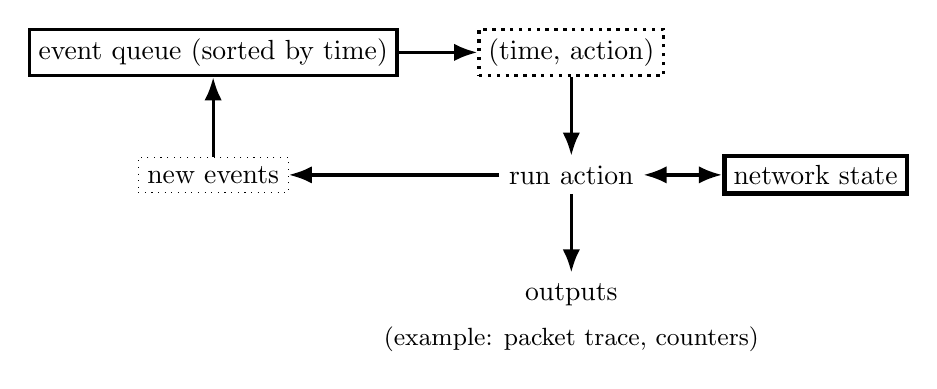
\begin{tikzpicture}
    % FIXME: queue --> event processing --> more things in queue
    % FIXME: show simulated clock
    % FIXME: show output list of events
    \node[draw,very thick] (queue) {event queue (sorted by time)};
    \node[draw,very thick,anchor=west,dotted] (next ev) at ([xshift=1cm]queue.east) {%
        (time, action)
    };
    \draw[very thick,-Latex] (queue) -- (next ev);
    \node[anchor=north] (run) at ([yshift=-1cm]next ev.south) {run action}; 
    \draw[very thick,-Latex] (next ev) -- (run);
    \node[anchor=west,draw, ultra thick] (network state) at ([xshift=1cm]run.east) {network state};
    \draw[very thick,Latex-Latex] (run) -- (network state);
    \node[draw,dotted] (new events) at (run.west -| queue.south) {new events};
    \draw[very thick,-Latex] (run.west) -- (new events);
    \draw[very thick,-Latex](new events) -- (queue.south);
    \draw[very thick,-Latex] (run.south) -- ++(0cm, -1cm) node[below] (outputs) {outputs};
    \node[anchor=north,font=\small] at (outputs.south) {(example: packet trace, counters)};
    % FIXME: second frame showing example event
\end{tikzpicture}
}{%
    Queue of events sorted by time and the latest event being pulled from the queue. The event pulled out of the queue
    is represented by a tuple of a time and an action. Running the action uses and updates a network state.
    Running the action yields new events, which are added back to the event queue, and outputs like packet traces
    and counters.
}
\end{frame}

\begin{frame}{action example 1}
\begin{itemize}
    \item take next packet from send queue for link X
    \item compute whether packet is lost due to error
    \item compute when packet is done transmitting
        \begin{itemize}
        \item schedule new event to handle next packet in queue at that time
    \end{itemize}
    \item compute reception time of packet on other end of link
        \begin{itemize}
        \item schedule new event to handle packet being received at that time
        \end{itemize}
\end{itemize}
\end{frame}

\begin{frame}{action example 2}
\begin{itemize}
    \item take next packet on link 0 of switch
    \item compute next link for packet
    \item add packet to queue for next link
    \item schedule new events:
        \begin{itemize}
        \item to dequeue from next link (if not scheduled already)
        \end{itemize}
\end{itemize}
\end{frame}
